\section{Étude de l'action de préhension \label{sec_5}}

\begin{obj}
L'objectif de cette partie est de valider les performances de serrage de la pince et de vérifier
les critères suivants du cahier des charges.
\begin{center}
\begin{tabular}{ll}
\hline
\textbf{Critère} & \textbf{Valeur} \\ \hline \hline
Diamètre des objets à saisir entre & \SI{40}{mm} et \SI{300}{mm} \\ \hline
Masse maximale des objets à saisir & \SI{2,5}{kg} \\
\hline
\end{tabular}
\end{center}
\end{obj}


\subsection{Actions mécaniques dans la pince}

\begin{obj}
Dans cette sous-partie, on établit la transmission des actions mécaniques entre
l'actionneur et l'effecteur et on quantifie les actions à fournir par l'actionneur pour respecter
le cahier des charges.
\end{obj}


La pince de préhension, servant à collecter les échantillons de roche ou à poser/prendre des
instruments sur le sol, est une pince à trois doigts (préhenseur tridigital, voir \autoref{fig_23}). Par
symétrie, on restreint l'étude à un seul doigt.
La chaîne cinématique correspondante est schématisée (modélisation plane) sur la \autoref{fig_23} ; elle
est constituée :
\begin{itemize}
\item du bâti 0 lié au bras manipulateur du système ROBOVOLC, auquel on associe le repère $\left(P,\vect{x_P},\vect{y_P},\vect{z_P}\right)$ avec
$\vect{x_P}$ la verticale descendante ;
\item  d'un vérin 1 en liaison glissière de direction $\vect{x_P}$ avec le bâti 0 ;
\item  d'une tige 2 en liaison pivot d'axe $\left(H,\vect{z_P}\right)$ avec le vérin 1 ;
\item  de deux biellettes 3 et 4 parallèles et en liaisons pivot d'axes respectifs $\left(A,\vect{z_P}\right)$ et $\left(C,\vect{z_P}\right)$
avec le bâti 0. La biellette 3 est également en liaison pivot d'axe $\left(E,\vect{z_P}\right)$ avec la tige 2 ;
\item  d'un mors 5 en liaisons pivot d'axes $\left(B,\vect{z_P}\right)$ et $\left(D,\vect{z_P}\right)$ avec les biellettes 3 et 4 ;
\item  d'un galet 6 en liaison rotule de centre $Q$ avec le mors 5 et en contact avec l'objet à saisir.
\end{itemize}
Les points $A$ , $B$ , $C$ , $D$ forment un parallélogramme. On introduit le paramétrage suivant :
$d=\vect{HP} \cdot \vect{y_P}=\vect{AP} \cdot \vect{y_P}=\vect{CP} \cdot \vect{y_P}$, 
$CE = EH = \ell_2$, 
$AC = BD = \ell_3$,
$AB = CD = \ell_4$,
$\vect{DQ} = L_5\vect{x_P} + \ell_5 \vect{y_P}$, 
$\vect{QS} = \ell_6\vect{y_P}$
ainsi que les angles
$\alpha = \left(\vect{HC},\vect{HE}\right)$
et  $\beta = \left(\vect{y_P},\vect{EC}\right)$.

On donne $d = \SI{50}{mm}$, $\ell_2 =\SI{100}{mm}$, $\ell_4 =\SI{150}{mm}$, $\ell_5 =\SI{20}{mm}$, $\ell_6 =\SI{15}{mm}$.

\begin{figure}[H]
\centering
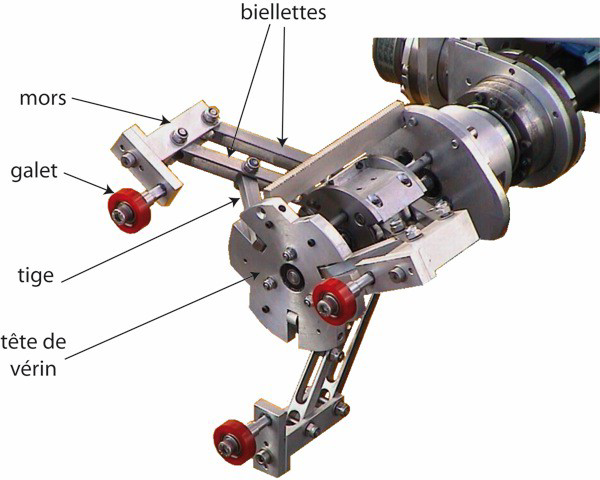
\includegraphics[width=.45\linewidth]{fig_23a.png}
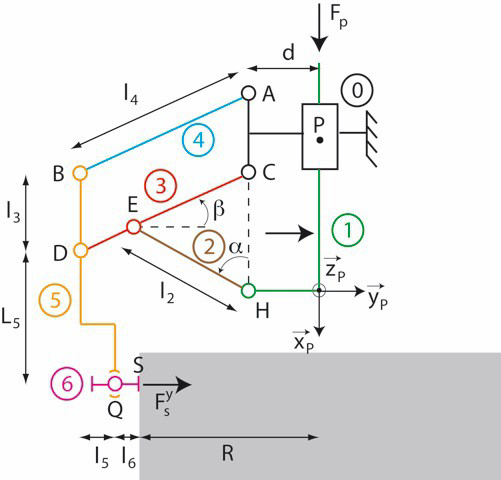
\includegraphics[width=.45\linewidth]{fig_23b.png}
\caption{Pince utilisée sur le système ROBOVOLC et schéma cinématique associé \label{fig_23}}
\end{figure}


Le contact entre le galet 6 et l'objet est modélisé par une liaison linéaire rectiligne d'axe $\left(S,\vect{x_P}\right)$ et
de normale $\vect{y_P}$ .
Dans une première approche, on considère que toutes les liaisons sont parfaites. De plus, le poids
des pièces composant la pince est négligé.
L'objet à saisir est modélisé par un cylindre à base circulaire de rayon $R$.


% Q5.1
\question{Donner le lien entre les angles $\alpha$ et $\beta$, ainsi que l'expression de ces angles en fonction du
rayon $R$ de l'objet et des données géométriques.}
\ifprof
\begin{corrige}
Une fermeture géométrique angulaire dans le triangle $CEH$ donne immédiatement :  $\alpha + \beta α+β=π/2

Une fermeture géométrique linéaire permet de déterminer la relation entre  α (ou β), R et les dimensions du mécanisme.
On trouve (en projetant sur l’axe x ⃗) :
R=d+l_4  cos⁡β-l_5-l_6
R=d+l_4  sin⁡α-l_5-l_6


\end{corrige}
\else
\fi

% Q5.2
\question{Montrer que la liaison équivalente entre le mors 5 et l'objet à saisir est une liaison ponctulle de normale $\left(S,\vect{y_P}\right)$. Cette liaison équivalente
sera utilisée dans la suite de cette partie.}
\ifprof
\begin{corrige}
\end{corrige}
\else
\fi

% Q5.3
%\question{Calculer l'hyperstatisme du modèle plan du mécanisme global de la pince (\autoref{fig_23}).}

% Q5.4
\question{Donner l'orientation de l'effort dans les liaisons pivot situées en $B$ et en $E$.}
\ifprof
\begin{corrige}
\end{corrige}
\else
\fi


L'ouverture/fermeture de la pince est réalisée par un moteur électrique et un système vis-écrou
fournissant un effort de poussée $\vect{F_P}=F_p\vect{x_P}$ sur le vérin 1 en amont de la pince. D'autre part, on
introduit à présent un modèle de frottement au contact entre le galet 6 et l'objet à saisir. Ce modèle
se traduit au niveau de la liaison équivalente entre le mors 5 et l'objet à saisir par un torseur
statique de la forme : $\torseurstat{T}{5}{\text{objet}}=\torseurl{-F_S^x\vect{x_P}+F_S^y\vect{y_P}}{\vect{0}}{S}$ 
où $F_S^x$ est l'effort tangentiel et $F_S^y$ est l'effort normal (ou de serrage) au contact.

% Q5.5
\question{Par une étude statique, montrer que les efforts $F_P$, $F_S^x$ et $F_S^y$ 
y sont liés par la relation $F_P = K \left( \tan \beta F_S^y - F_S^x\right)$  
où l'expression de la constante $K$ est à préciser en fonction de $\ell_2$ et $\ell_4$.
Montrer également que cette relation est indépendante de la longueur $L_5$ et expliquer l'avantage technique de ce résultat.}
\ifprof
\begin{corrige}
\end{corrige}
\else
\fi

On représente sur la \autoref{fig_24}  l'évolution de $\tan \beta$ en fonction du rayon $R$ de l'objet à saisir sur la plage $R =[\SI{20}{mm}, \SI{165}{mm}]$.

\begin{figure}[H]
\centering
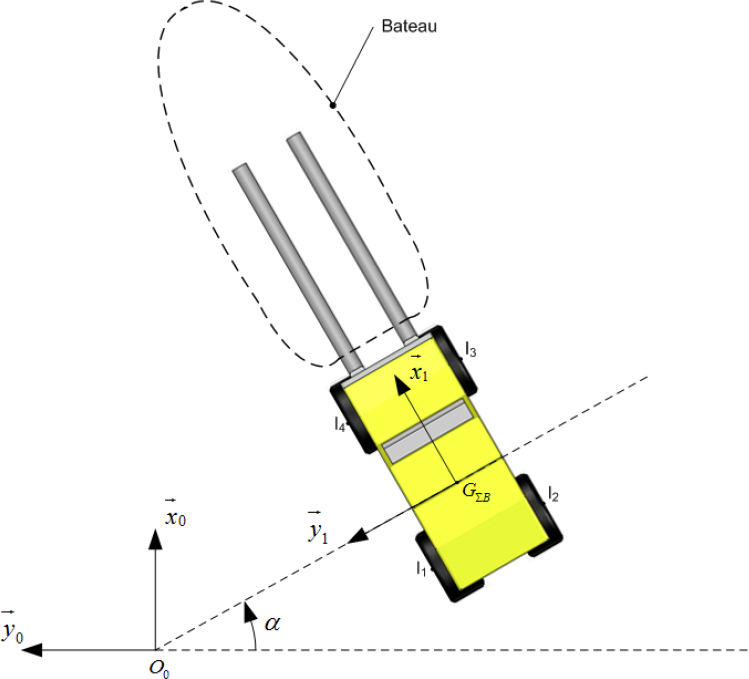
\includegraphics[width=10cm]{fig_24.png}
\caption{Evolution de $\tan \beta$ en fonction de $R$ \label{fig_24}}
\end{figure}


%Q5.6 : 
\question{Commenter ce graphe, en particulier pour les valeurs extrêmes du rayon $R$.}
\ifprof
\begin{corrige}
\end{corrige}
\else
\fi

%Q5.7 : 
\question{En supposant un modèle de frottement de Coulomb (le coefficient de frottement est noté $f$), 
montrer que l'objet peut être saisi et soulevé sans aucune action de poussée $F_p$ du moteur
lorsque le rayon de l'objet est tel que $R \geq R_{\text{min}}$. On précisera l'expression de $ R_{\text{min}}$ , on donnera sa
valeur pour $f =2$, et on commentera ce caractère particulier de la pince en donnant un avantage
et un inconvénient.}
\ifprof
\begin{corrige}
\end{corrige}
\else
\fi

%Q5.8 : 
\question{Pour $R < R_{\text{min}}$, donner la relation entre l'effort de poussée $F_p$ et la masse $m_{\text{objet}}$ de l'objet
à saisir, ainsi qu'entre l'effort de poussée $F_p$ et l'effort de serrage$F_S^y$ . En déduire la valeur de
l'effort de poussée maximal à fournir pour respecter le cahier des charges avec $f =2$.}
\ifprof
\begin{corrige}
\end{corrige}
\else
\fi

\subsection{Asservissement de l'effort}

\begin{obj}
Dans cette sous-partie, on étudie l’asservissement en effort de la pince. En lien avec la
sous-partie précédente, on se place dans la configuration $R < R_{\text{min}}$ et on donne la relation
$F_s^y = K_{\beta} F_p$.
\end{obj}


La pince a un capteur d'effort pour mesurer et contrôler la force de serrage. Pour l'asservissement
de la pince, une régulation en effort est faite. Le schéma bloc de la \autoref{fig_25} présente la structure
de contrôle de la pince.


\begin{figure}[H]
\centering
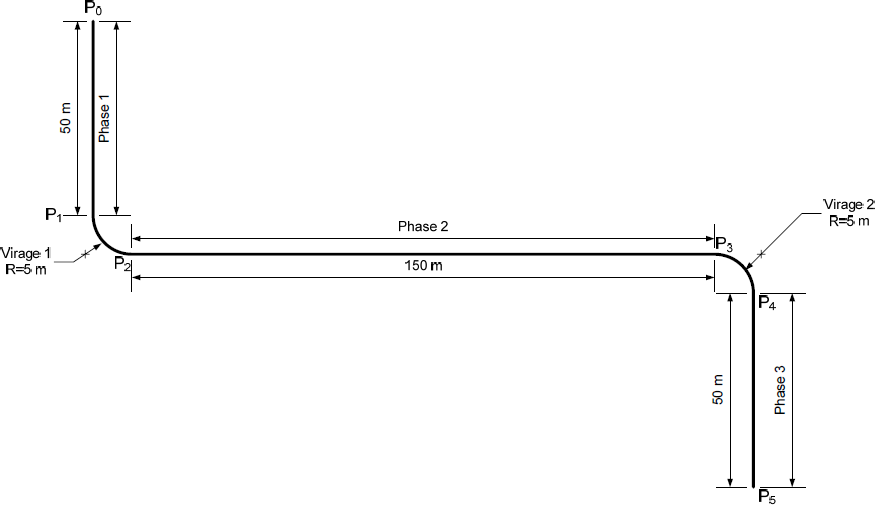
\includegraphics[width=.9\linewidth]{fig_25.png}
\caption{Schéma d'asservissement \label{fig_25}}
\end{figure}


%Q5.9 : 
\question{Quel est l'intérêt pratique de la régulation mise en place ?}


Pour l’étude en asservissement de la pince, on fixe $K_{\beta} = 2,2$.
On donne les caractéristiques du système suivantes.

\begin{table}[H]
\centering
\begin{tabular}{lll}
\hline
$R$ &  résistance d'induit 		& $\SI{7,2}{\Omega}$ \\ \hline
$L$ &   inductance d'induit 	& \SI{2,56}{mH} \\ \hline
$K_t$ &  constante de couple 	& \SI{0,82}{Nm/A} \\ \hline
$K_e$ &  constante de fcem 	& \SI{86}{V/1000tr/min} \\ \hline
$J_{\text{eq}}$ &  moment d'inertie 	& \SI{3,45e-4}{ kg m^2} \\ \hline
$Kr$ &  rapport du réducteur 	& $54/33=1,636$ \\ \hline
$K_{\text{ve}}$ & pas du système vis-écrou & $\SI{4}{mm}$  \\ \hline
\end{tabular}
\end{table}


%Q5.10 : 
\question{En considérant $P_F=0$ (perturbation nulle) et $L=0$ (inductance nulle), calculer la fonction de transfert
$\dfrac{F_S^y}{F_c}$ et la mettre sous la forme canonique $\dfrac{K}{1+Ap+Bp^2}$. Identifier les paramètres $K$,
$A$ et $B$.}
\ifprof
\begin{corrige}
\end{corrige}
\else
\fi

On souhaite une erreur de position inférieure à 1\%.

%Q5.11 : 
\question{Calculer la valeur de $C_f$ permettant de respecter cette contrainte.}
\ifprof
\begin{corrige}
\end{corrige}
\else
\fi

%Q5.12: 
\question{Bien qu’il y ait un intégrateur dans la chaîne directe, indiquer pourquoi l’erreur statique est non-nulle.}
\ifprof
\begin{corrige}
\end{corrige}
\else
\fi

%Q5.13: 
\question{En considérant une valeur du correcteur permettant de valider le critère d’erreur de
position, ce critère sera-t-il toujours validé si on ne néglige plus les perturbations ? Comment le
démontrer ?}

%Q5.14: 
\question{Le coefficient  $K_{\beta}$ a-t-il une influence sur l’asservissement ? Pourquoi ne peut-on pas
considérer $K_{\beta}$ comme une constante ?}
\ifprof
\begin{corrige}
\end{corrige}
\else
\fi

Pour des raisons techniques, il n'est pas possible d'utiliser un capteur d'effort en bout de pince.

%Q5.15 : 
\question{Est-il techniquement possible d'asservir le système sans ce capteur d'effort ? Expliquer le
raisonnement.}
\ifprof
\begin{corrige}
\end{corrige}
\else
\fi

Dans l'étude précédente, la masse de l'objet et le coefficient de frottement entre la pince et l'objet
sont supposés connus. Cependant, ce n’est pas le cas en pratique et il peut en résulter un
glissement possible de l’objet si ces paramètres sont mal évalués.

%Q5.16 : 
\question{Quel moyen peut-on imaginer afin de limiter le glissement de l’objet ? Expliquer le
raisonnement.}
\ifprof
\begin{corrige}
\end{corrige}
\else
\fi

